\chapter{Fermionen, Dirac-Matrizen und das Dirac-Meer}

Das Dirac-Meer ist unser Ziel, doch auch der Weg dorthin ist wichtig. Bevor wir uns der negativen Energie in der relativistischen Elektronentheorie zuwenden, benötigen wir zwei mathematische Werkzeuge. Zunächst betrachten wir die Operatoralgebra, die Fermionen von Bosonen unterscheidet. Danach wiederholen wir die eindimensionale Dirac-Gleichung, in der sich jede Erweiterung der Wellenfunktion erkennen lässt, ohne dass die Geometrie dreier Raumdimensionen hinzukommt. Sind diese Grundlagen geschaffen, erzwingt die dreidimensionale Gleichung ihre eigene Matrixstruktur. Die einleitende Betrachtung besetzter und leerer Fermionenzustände wird dann als Schlüssel zum Verständnis der Positronen wieder aufgegriffen.

Wir verwenden \(c=\hbar=1\). Das große \(P\) bezeichnet einen Impulsoperator, das kleine \(p\) einen Impulseigenwert und die fettgedruckten Symbole deren dreidimensionale Versionen.

\section{Austausch wird zur Operatoralgebra}

Betrachten wir zwei identische Teilchen, eines bei \(x\) und eines bei \(y\). Die Bezeichnungen \(x\) und \(y\) stehen für vollständige Ortsangaben; sie sind nicht zwei kartesische Koordinaten eines einzelnen Teilchens. Die Wirkung zweier Erzeugungsoperatoren auf das Vakuum ergibt
\begin{equation}
\lvert x,y\rangle
=
\psi^\dagger(x)\psi^\dagger(y)\lvert0\rangle.
\label{eq:l10-two-particle-state}
\end{equation}

Bei Bosonen bleibt der Zustand beim Vertauschen der beiden Plätze unverändert:
\begin{equation}
\lvert x,y\rangle=\lvert y,x\rangle.
\end{equation}
Die Operatorgleichung, die diese Symmetrie sicherstellt, lautet
\begin{equation}
\psi^\dagger(x)\psi^\dagger(y)
=
\psi^\dagger(y)\psi^\dagger(x).
\label{eq:l10-boson-exchange}
\end{equation}
Zwei bosonische Erzeugungsoperatoren kommutieren. Daher können wir ihre Reihenfolge umkehren, ohne den von ihnen erzeugten Zustand zu ändern.

Bei Fermionen ändert der Austausch das Vorzeichen:
\begin{equation}
\lvert x,y\rangle=-\lvert y,x\rangle.
\label{eq:l10-fermion-state-exchange}
\end{equation}
Das Gesamtvorzeichen eines einzelnen Zustandsvektors ist nicht beobachtbar, relative Vorzeichen zwischen Alternativen hingegen schon. Deshalb muss dieses Minuszeichen durchgehend beibehalten werden. Gleichung~\eqref{eq:l10-fermion-state-exchange} verlangt
\begin{equation}
\psi^\dagger(x)\psi^\dagger(y)
=
-\,\psi^\dagger(y)\psi^\dagger(x).
\label{eq:l10-fermion-operator-exchange}
\end{equation}

\begin{figure}[htbp]
\centering
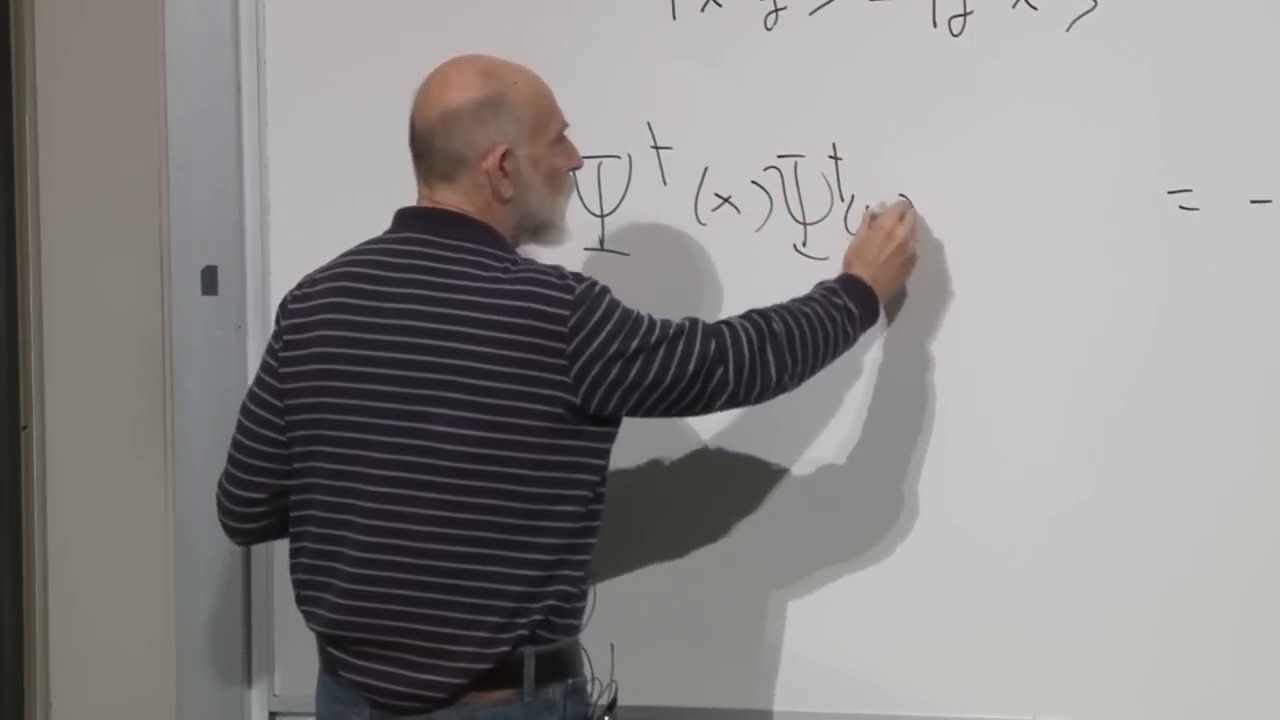
\includegraphics[width=0.94\linewidth]{lecture_10_figure_02.png}
\caption{Die Tafelgleichung, die den Austausch von Fermionen beschreibt. Beim Vertauschen der Erzeugungsoperatoren ändert der Zweiteilchenzustand sein Vorzeichen.}
\lectureframe{00:05:50}
\end{figure}

Für zwei beliebige Operatoren \(A\) und \(B\) definieren wir den Antikommutator durch
\begin{equation}
\{A,B\}:=AB+BA.
\end{equation}
Die Austauscherelation lautet folglich
\begin{equation}
\{\psi^\dagger(x),\psi^\dagger(y)\}=0.
\label{eq:l10-creation-anticommutator}
\end{equation}
In der entsprechenden Fermionenfeldalgebra treten an die Stelle der bosonischen Kommutatoren Antikommutatoren. Die beiden Verwendungen des Wortes „antikommutieren“ müssen auseinandergehalten werden: Feldoperatoren antikommutieren aufgrund der Fermi-Statistik, während Matrizen später antikommutieren, damit sich die Kreuzterme in einer relativistischen Dispersionsrelation aufheben.

Setzen wir nun \(y=x\) in Gleichung~\eqref{eq:l10-creation-anticommutator} ein. Beide Produkte sind dann gleich:
\begin{align}
0
&=\{\psi^\dagger(x),\psi^\dagger(x)\}\\
&=2\,\psi^\dagger(x)\psi^\dagger(x).
\end{align}
Also gilt
\begin{equation}
\bigl(\psi^\dagger(x)\bigr)^2=0.
\label{eq:l10-exclusion}
\end{equation}
Versucht man, zwei identische Fermionen im selben Einteilchenzustand zu erzeugen, erhält man den Nullvektor. Das ist das Pauli-Ausschlussprinzip in Operatorform.

\begin{figure}[htbp]
\centering
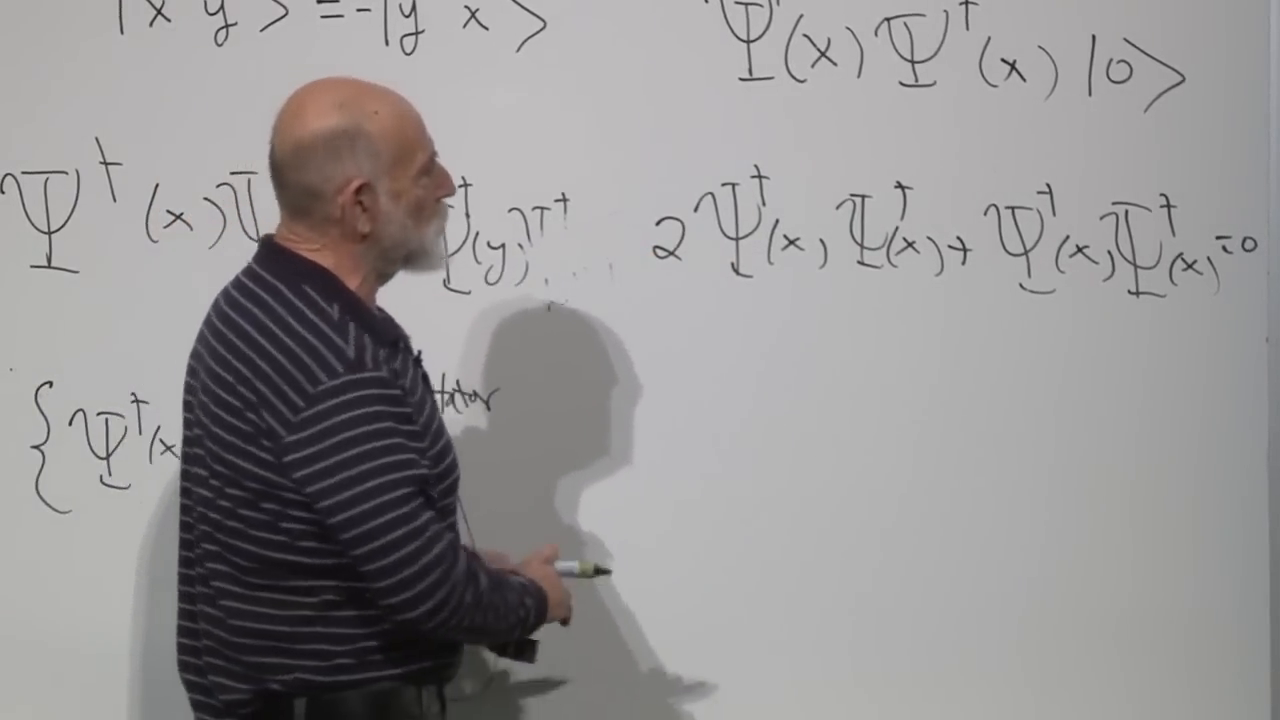
\includegraphics[width=0.94\linewidth]{lecture_10_figure_03.png}
\caption{Der Spezialfall gleicher Zustände an der Tafel. Das wiederholte Produkt der Erzeugungsoperatoren tritt zweimal auf und muss daher verschwinden.}
\lectureframe{00:08:04}
\end{figure}

\begin{figure}[htbp]
\centering
\begin{adjustbox}{max width=\linewidth}
\begin{tikzpicture}[node distance=1.25cm,>=Latex]
\node[draw,rounded corners,align=center,inner sep=7pt] (a)
  {$\{\psi^\dagger(x),\psi^\dagger(x)\}=0$};
\node[draw,rounded corners,align=center,inner sep=7pt,right=of a] (b)
  {$2(\psi^\dagger(x))^2=0$};
\node[draw,rounded corners,align=center,inner sep=7pt,right=of b] (c)
  {$(\psi^\dagger(x))^2=0$};
\draw[->,thick] (a) -- (b);
\draw[->,thick] (b) -- (c);
\end{tikzpicture}
\end{adjustbox}
\caption{Das Ausschlussargument, rekonstruiert ohne die teilweise ausgewischten Zwischenschritte an der Tafel.}
\end{figure}

\section{Warum bei Fermionen besetzt und leer symmetrisch sind}

Zwischen bosonischen und fermionischen Operatoren gibt es einen zweiten Unterschied, der subtiler ist als das Ausschlussprinzip und später wesentlich wird. Für einen einzelnen bosonischen Modus gilt
\begin{equation}
[a,a^\dagger]=1,
\qquad
n=0,1,2,\ldots.
\end{equation}
Beim Vertauschen von \(a\) und \(a^\dagger\) ändert sich das Vorzeichen des Kommutators. Selbst wenn die Operatoren lediglich \(A\) und \(B\) hießen, würde die Algebra verraten, welche Reihenfolge die Besetzungszahl erhöht und welche sie verringert.

Auch die bosonische Besetzungsleiter hat eine Orientierung. Der Vernichtungsoperator erreicht schließlich \(\lvert0\rangle\) und wirkt darauf mit null, während der Erzeugungsoperator unbegrenzt weiterwirken kann:
\begin{align}
a\lvert0\rangle&=0,\\
a^\dagger\lvert n\rangle&\propto\lvert n+1\rangle,
\qquad n=0,1,2,\ldots.
\end{align}
Kehrt man diese Leiter um, erhält man nicht dasselbe Spektrum. Es gibt eine untere Grenze, aber keine obere.

Für einen einzelnen fermionischen Modus gilt
\begin{equation}
\{a,a^\dagger\}=1,
\qquad
a^2=(a^\dagger)^2=0,
\qquad
n=0,1.
\label{eq:l10-fermion-mode}
\end{equation}
Der Erzeugungsoperator überführt den leeren Zustand in den besetzten Zustand und wirkt danach mit null:
\begin{equation}
a^\dagger\lvert0\rangle=\lvert1\rangle,
\qquad
a^\dagger\lvert1\rangle=0.
\end{equation}
Der Vernichtungsoperator bewirkt die Umkehrung:
\begin{equation}
a\lvert1\rangle=\lvert0\rangle,
\qquad
a\lvert0\rangle=0.
\end{equation}
Es gibt nur zwei Zustände. Daher ist das Diagramm unter dem Vertauschen von „besetzt“ und „leer“ sowie von \(a\) und \(a^\dagger\) symmetrisch. Die Operatoren haben weiterhin unterschiedliche physikalische Bedeutungen, doch ihre Algebra zeichnet den einen nicht mehr als Erzeugungsoperator und den anderen als Vernichtungsoperator aus. Diese formale Symmetrie bildet den Ausgangspunkt für die Teilchen-Loch-Umdeutung.

\begin{classroomqa}
\lecturetimestamp{00:13:54}
\audiencequestion{Wenn \((a^\dagger)^2=0\) gilt, ist das ein Widerspruch, oder folgt daraus, dass \(a^\dagger=0\)?}
\lecturerresponse{Weder noch. Ein von null verschiedener Operator kann ein verschwindendes Quadrat haben. Hier überführt \(a^\dagger\) den Zustand \(\lvert0\rangle\) in \(\lvert1\rangle\), doch oberhalb von \(\lvert1\rangle\) gibt es keinen erlaubten Zustand. Zweimalige Anwendung ergibt daher null. Dieselbe Überlegung liefert \(a^2=0\).}
\end{classroomqa}

Behalten wir diese Symmetrie zwischen besetzt und leer im Hinterkopf. Wenn später ein Elektron mit negativer Energie entfernt wird, wird der Vernichtungsoperator als Erzeugungsoperator eines Positrons umgedeutet. Das ist keine willkürliche Änderung der Bezeichnung; sie nutzt genau die hier hergeleitete Zweizustandsalgebra der Fermionen.

\section{Die eindimensionale Dirac-Konstruktion}

Kehren wir nun zu einem Teilchen in einer Raumdimension zurück. Die einfachste relativistische Wellengleichung erster Ordnung lautet
\begin{equation}
i\partial_t\psi=-\,i\partial_x\psi.
\label{eq:l10-right-mover}
\end{equation}
Mit \(P=-i\partial_x\) wird daraus
\begin{equation}
H=P.
\end{equation}
Für einen Impulseigenzustand gilt \(E=p\), und seine Gruppengeschwindigkeit ist
\begin{equation}
v_g=\frac{dE}{dp}=1.
\end{equation}
Sowohl bei positivem als auch bei negativem Impuls und damit bei positiver wie negativer Energie bewegt sich die Welle weiterhin starr nach rechts. Das Vorzeichen von \(p\) ändert das Phasenmuster, nicht die Ausbreitungsrichtung.

Ein massives Teilchen muss sich in beide Richtungen bewegen können. Wir führen eine zweite Komponente ein, die folgende Gleichung erfüllt:
\begin{equation}
H\psi_1=P\psi_1,
\qquad
H\psi_2=-P\psi_2.
\label{eq:l10-two-directions}
\end{equation}
Die erste Komponente bewegt sich nach rechts, die zweite nach links. Wir fassen sie zu einem Spaltenvektor zusammen,
\begin{equation}
\Psi=
\begin{pmatrix}
\psi_1\\
\psi_2
\end{pmatrix},
\end{equation}
und definieren
\begin{equation}
\alpha=
\begin{pmatrix}
1&0\\
0&-1
\end{pmatrix}.
\end{equation}
Damit lassen sich beide Gleichungen schreiben als
\begin{equation}
H\Psi=\alpha P\Psi.
\label{eq:l10-massless-one-d}
\end{equation}
Für die Berücksichtigung beider Richtungen kommt ein neuer zweifachwertiger innerer Freiheitsgrad hinzu.

Die Richtung allein führt noch nicht zur Masse. Wir führen eine zweite Matrix ein,
\begin{equation}
\beta=
\begin{pmatrix}
0&1\\
1&0
\end{pmatrix},
\end{equation}
und setzen an:
\begin{equation}
H=\alpha P+\beta m.
\label{eq:l10-massive-one-d}
\end{equation}
Die Matrizen erfüllen
\begin{equation}
\alpha^2=\beta^2=\mathbb{1},
\qquad
\{\alpha,\beta\}=0.
\label{eq:l10-one-d-algebra}
\end{equation}
Durch Quadrieren des Hamiltonoperators erhalten wir
\begin{align}
H^2
&=(\alpha P+\beta m)^2\\
&=\alpha^2P^2+\beta^2m^2
  +(\alpha\beta+\beta\alpha)Pm\\
&=P^2+m^2.
\label{eq:l10-one-d-dispersion}
\end{align}
Der Antikommutator in Gleichung~\eqref{eq:l10-one-d-algebra} beseitigt den unerwünschten Term, der sowohl von \(P\) als auch von \(m\) linear abhängt.

Die Nebendiagonalmatrix \(\beta\) koppelt die beiden Richtungskomponenten. Man kann sich vorstellen, dass der Massenterm rechts- und linkslaufende Amplituden fortwährend miteinander mischt. Dieses Bild sollte nicht wörtlich als ein Teilchen verstanden werden, das auf einer mikroskopischen Bahn hin und her springt. Es macht jedoch anschaulich, warum ein massives Wellenpaket eine mittlere Geschwindigkeit unterhalb der Lichtgeschwindigkeit haben und ein Ruhesystem besitzen kann, während dies für eine isolierte masselose chirale Komponente nicht möglich ist.

\begin{classroomqa}
\lecturetimestamp{00:23:37}
\audiencequestion{Gibt es eine tiefergehende physikalische Deutung dafür, dass beide Richtungskomponenten eingeführt werden?}
\lecturerresponse{Ja, doch in drei Dimensionen wird sie deutlicher. Hier sind sie zunächst einfach die beiden Komponenten, die nötig sind, um entgegengesetzte Ausbreitungsrichtungen zu beschreiben und eine Massenkopplung über die Nebendiagonale zu ermöglichen. Ihre spätere Deutung lautet Händigkeit oder Chiralität.}
\end{classroomqa}

\section{Drei Dimensionen erzwingen die Pauli-Matrizen}

In drei Raumdimensionen ist der Impuls ein Vektor. Ein in ihm linearer Hamiltonoperator, der ein Rotationsskalar ist, legt daher einen weiteren Vektor nahe, dessen Komponenten nun Matrizen sind:
\begin{equation}
H=\boldsymbol{\alpha}\cdot\mathbf P
=\alpha_xP_x+\alpha_yP_y+\alpha_zP_z.
\label{eq:l10-three-d-ansatz}
\end{equation}

\begin{figure}[htbp]
\centering
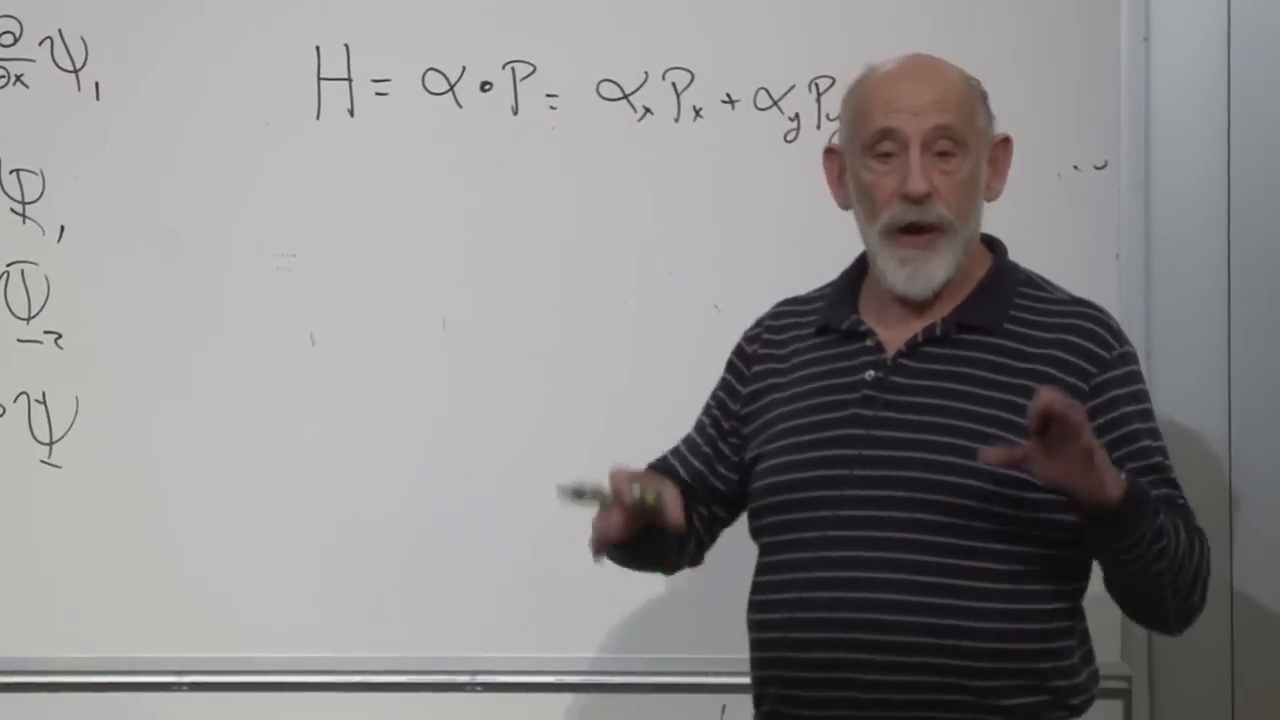
\includegraphics[width=0.94\linewidth]{lecture_10_figure_04.png}
\caption{Der dreidimensionale masselose Ansatz \(H=\boldsymbol{\alpha}\cdot\mathbf P\) an dem Punkt, an dem eine Matrix durch einen Vektor aus drei Matrizen ersetzt wird.}
\lectureframe{00:26:00}
\end{figure}

Beginnen wir erneut mit dem masselosen Fall. Wir verlangen
\begin{equation}
H^2=\mathbf P^2=P_x^2+P_y^2+P_z^2.
\end{equation}
Quadrieren wir Gleichung~\eqref{eq:l10-three-d-ansatz} und entwickeln das Ergebnis,
\begin{align}
H^2
&=\alpha_x^2P_x^2+\alpha_y^2P_y^2\\
&\quad+\alpha_z^2P_z^2\\
&\quad+\{\alpha_x,\alpha_y\}P_xP_y\\
&\quad+\{\alpha_x,\alpha_z\}P_xP_z\\
&\quad+\{\alpha_y,\alpha_z\}P_yP_z.
\end{align}
so stimmen die Diagonalterme, wenn
\begin{equation}
\alpha_x^2=\alpha_y^2=\alpha_z^2=\mathbb{1},
\end{equation}
gilt, und sämtliche Kreuzterme verschwinden, wenn
\begin{equation}
\{\alpha_i,\alpha_j\}=0,
\qquad i\ne j.
\label{eq:l10-alpha-anticommutation}
\end{equation} gilt.

Drei bekannte \(2\times2\)-Matrizen erfüllen genau diese Bedingungen:
\begin{equation}
\sigma_x=
\begin{pmatrix}
0&1\\
1&0
\end{pmatrix},
\quad
\sigma_y=
\begin{pmatrix}
0&-i\\
i&0
\end{pmatrix},
\quad
\sigma_z=
\begin{pmatrix}
1&0\\
0&-1
\end{pmatrix}.
\label{eq:l10-pauli-matrices}
\end{equation}
Eine Lösung lautet also
\begin{equation}
\alpha_i=\sigma_i,
\qquad
H=\boldsymbol{\sigma}\cdot\mathbf P.
\label{eq:l10-weyl-hamiltonian}
\end{equation}

\begin{figure}[htbp]
\centering
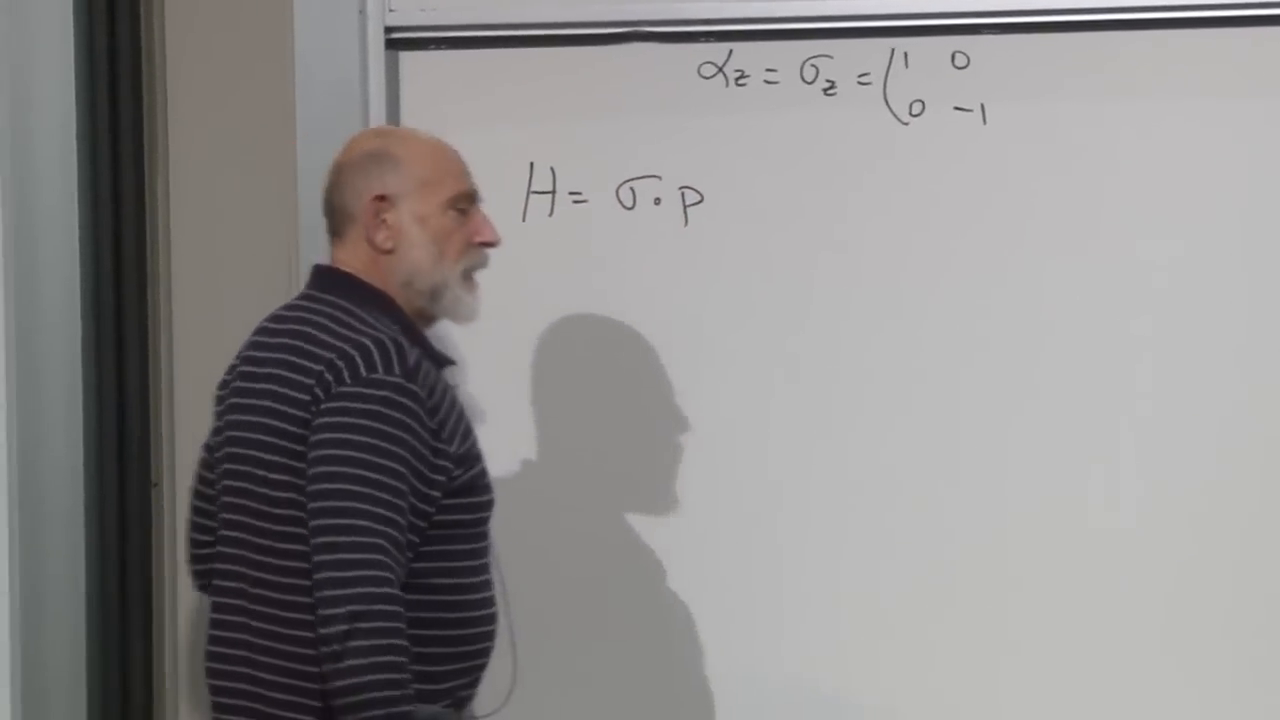
\includegraphics[width=0.94\linewidth]{lecture_10_figure_05.png}
\caption{Der kompakte masselose Hamiltonoperator \(H=\boldsymbol{\sigma}\cdot\mathbf P\), mit dem darüber weiterhin sichtbaren \(\alpha_z=\sigma_z\).}
\lectureframe{00:28:16}
\end{figure}

Für einen Impulseigenzustand gilt
\begin{equation}
\boldsymbol{\sigma}\cdot\mathbf p
=
|\mathbf p|\,\boldsymbol{\sigma}\cdot\widehat{\mathbf p}.
\end{equation}
Der Operator \(\boldsymbol{\sigma}\cdot\widehat{\mathbf p}\) hat die Eigenwerte \(+1\) und \(-1\). Daher gilt
\begin{equation}
E=\pm|\mathbf p|.
\end{equation}
In dieser Zweikomponententheorie ist bei positiver Energie der Pauli-Freiheitsgrad am Impuls ausgerichtet, bei negativer Energie dagegen entgegengesetzt zu ihm. Diese Ausrichtung ist festgelegt; bei gegebenem Vorzeichen der Energie lässt sich die Spinrichtung nicht unabhängig davon wählen.

\begin{classroomqa}
\lecturetimestamp{00:30:10}
\audiencequestion{Ergibt sich der Spin aus der Dirac-Gleichung, oder wurde er eingeführt, weil bereits bekannt war, dass das Elektron ein magnetisches Moment hat?}
\lecturerresponse{Hier bedeutet „sich ergeben“: „als Folge hervorgehen“, nicht „verschwinden“. Ausgangspunkt war die Forderung nach einem in den Impulskomponenten linearen Hamiltonoperator, dessen Quadrat \(\mathbf P^2\) ist. Gewöhnliche Zahlen können die verlangte Algebra nicht erfüllen, die Pauli-Matrizen hingegen schon. Ihre Zweikomponentenstruktur ergibt sich daher bereits aus der Linearisierung selbst. Das beweist nicht, dass jedes Teilchen Spin haben muss; es besagt, dass Teilchen, die durch diese Dirac-artige Gleichung beschrieben werden, den entsprechenden Spinor-Freiheitsgrad besitzen.}
\end{classroomqa}

Dies ist eine der zentralen Lehren dieser Konstruktion. Die Matrizen sind keine dekorativen Bezeichnungen, die nachträglich zur relativistischen Gleichung hinzugefügt werden. Sie entstehen beim Versuch, eine lokale Quadratwurzel der relativistischen Dispersionsrelation zu bilden.

\section{Warum die Masse vier Komponenten erfordert}

Versuchen wir, die eindimensionale Massenkonstruktion zu wiederholen, ohne die \(2\times2\)-Theorie zu erweitern:
\begin{equation}
H=\boldsymbol{\sigma}\cdot\mathbf P+\beta m.
\label{eq:l10-failed-mass}
\end{equation}
Wir nehmen \(\beta^2=\mathbb{1}\) an. Das Quadrat enthält zwar die gewünschten Terme \(\mathbf P^2+m^2\), aber auch
\begin{equation}
m\sum_i\{\sigma_i,\beta\}P_i.
\end{equation}
Um diesen Term zu beseitigen, müsste eine Matrix \(\beta\) die Bedingung
\begin{equation}
\{\sigma_x,\beta\}
=
\{\sigma_y,\beta\}
=
\{\sigma_z,\beta\}
=0.
\label{eq:l10-impossible-beta}
\end{equation}
erfüllen. Es gibt keine Matrix der Größe \(2\times2\) mit dieser Eigenschaft. Die Einheitsmatrix kommutiert mit allen drei Pauli-Matrizen, und jede spurlose Matrix der Größe \(2\times2\) ist eine Linearkombination der Pauli-Matrizen. Jede solche Kombination antikommutiert nicht mit der Komponente, die parallel zu ihr ist. In der \(2\times2\)-Algebra gibt es keine vierte unabhängige Matrix der benötigten Art.

Abhilfe schafft eine Erweiterung des Spinors. Vier Matrizen, die paarweise antikommutieren und deren Quadrate die Einheitsmatrix sind, treten erstmals in einer komplexen Darstellung der Größe \(4\times4\) auf. Diese Matrixgröße wurde nicht deshalb gewählt, weil die Raumzeit vier Dimensionen hat; sie ist der kleinste Matrizenraum, in dem sich die geforderte Algebra realisieren lässt.

Es gibt viele äquivalente Darstellungen. Eine unitäre Änderung der Spinorbasis verändert die Einträge sämtlicher Matrizen, ohne eine physikalische Vorhersage zu ändern. Entscheidend ist die abstrakte Menge der Relationen
\begin{equation}
\{\alpha_i,\alpha_j\}=2\delta_{ij}\mathbb{1},
\qquad
\{\alpha_i,\beta\}=0,
\qquad
\beta^2=\mathbb{1}.
\label{eq:l10-dirac-algebra}
\end{equation}

\begin{classroomqa}
\lecturetimestamp{00:37:38}
\audiencequestion{Kann man \(\beta\) als Zeitkomponente \(\alpha_t\) auffassen?}
\lecturerresponse{Nicht unmittelbar. Die drei \(\alpha_i\) bilden mit \(\beta\) nicht die vier Komponenten eines einzigen Lorentz-Vektors. In kovarianter Notation definiert man stattdessen \(\beta=\gamma^0\) und \(\alpha_i=\gamma^0\gamma^i\); die vier Matrizen \(\gamma^\mu\) erfüllen die Raumzeit-Clifford-Algebra.}
\end{classroomqa}

Eine praktische Blockdarstellung ist
\begin{equation}
\alpha_i=
\begin{pmatrix}
\sigma_i&0\\
0&-\sigma_i
\end{pmatrix},
\qquad
\beta=
\begin{pmatrix}
0&I_2\\
I_2&0
\end{pmatrix}.
\label{eq:l10-block-representation}
\end{equation}
Die Pauli-Matrizen in den Diagonalblöcken gewährleisten, dass verschiedene \(\alpha_i\) antikommutieren. Die Einheitsmatrizen in den Nebendiagonalblöcken von \(\beta\) gewährleisten, dass \(\beta\) mit jedem \(\alpha_i\) antikommutiert.

\begin{figure}[htbp]
\centering
\includegraphics[width=0.94\linewidth]{lecture_10_figure_06.png}
\caption{Die Blockdarstellung der Größe \(4\times4\) an der Tafel. Die oberen Gleichungen geben die geforderten Antikommutatoren an; die vollständigen Matrizen sind in Gleichung~\eqref{eq:l10-block-representation} gesetzt.}
\lectureframe{00:41:10}
\end{figure}

Der massive Hamiltonoperator lautet nun
\begin{equation}
H=\boldsymbol{\alpha}\cdot\mathbf P+\beta m
=
\begin{pmatrix}
\boldsymbol{\sigma}\cdot\mathbf P&mI_2\\
mI_2&-\boldsymbol{\sigma}\cdot\mathbf P
\end{pmatrix}.
\label{eq:l10-massive-dirac}
\end{equation}
Unter Verwendung von Gleichung~\eqref{eq:l10-dirac-algebra} erhalten wir
\begin{equation}
H^2=\mathbf P^2+m^2.
\end{equation}
Die Vierkomponentenstruktur ist also keine optionale Ergänzung. Sie ist die kleinste Struktur, die sowohl einen dreidimensionalen Impuls als auch einen Massenterm zulässt und zugleich die Gleichung erster Ordnung erhält.

\section{Chiralität und die Bedeutung der zusätzlichen Komponenten}

Welche physikalische Unterscheidung kommt durch die Erweiterung hinzu? Betrachten wir zunächst den masselosen oberen Block,
\begin{equation}
H_R=\boldsymbol{\sigma}\cdot\mathbf P,
\end{equation}
und den masselosen unteren Block,
\begin{equation}
H_L=-\boldsymbol{\sigma}\cdot\mathbf P.
\end{equation}
Bei Zuständen mit positiver Energie ist im ersten Block der Spin am Impuls ausgerichtet, im zweiten dagegen entgegengesetzt. Es handelt sich um entgegengesetzte Helizitäten. In einer masselosen Theorie bleibt die Helizität unter eigentlichen Lorentz-Transformationen invariant, denn kein Beobachter kann ein lichtartiges Teilchen überholen und dessen Impuls umkehren, während sein Spin unverändert bleibt. Die beiden Blöcke beschreiben daher entgegengesetzte chirale Sektoren.

\begin{classroomqa}
\lecturetimestamp{00:41:28}
\audiencequestion{In einer Dimension war ein zusätzlicher binärer Freiheitsgrad nötig, um Masse einzuführen. Welche physikalische Unterscheidung entspricht ihm in drei Dimensionen?}
\lecturerresponse{Es ist die Händigkeit des Spinors. Die beiden Blöcke der Größe \(2\times2\) beschreiben entgegengesetzte Beziehungen zwischen Spin und Impuls. Der eine ist rechtshändig, der andere linkshändig. Die Theorie mit Matrizen der Größe \(4\times4\) umfasst beide.}
\end{classroomqa}

Der Massenterm in Gleichung~\eqref{eq:l10-massive-dirac} steht außerhalb der Diagonale. Er überführt eine Amplitude des oberen Blocks in den unteren Block und umgekehrt:
\begin{equation}
\beta m
\begin{pmatrix}
\Psi_R\\
\Psi_L
\end{pmatrix}
=
m
\begin{pmatrix}
\Psi_L\\
\Psi_R
\end{pmatrix}.
\end{equation}
Masse koppelt also entgegengesetzte Chiralitäten miteinander.

\begin{classroomqa}
\lecturetimestamp{00:43:58}
\audiencequestion{Kann ein masseloses Teilchen seine Chiralität ändern?}
\lecturerresponse{Nicht unter dem hier gezeigten freien masselosen Hamiltonoperator. Die beiden Blöcke sind entkoppelt, sodass ein anfangs rechts- oder linkshändiger Zustand dies auch bleibt. Genau der Nebendiagonalterm für die Masse mischt die beiden, wenn \(m\ne0\) gilt.}
\end{classroomqa}

Diese Aussage ist für die Blockdarstellung exakt. Das Bild eines Teilchens, das mechanisch zwischen zwei Pfeilen hin- und herwechselt, sollte man jedoch nicht überstrapazieren. Die physikalische Aussage ist die Matrixkopplung in der Wellengleichung.

\begin{classroomqa}
\lecturetimestamp{00:44:50}
\audiencequestion{Sind diese Matrizen in den Quaternionen angelegt?}
\lecturerresponse{Die Pauli-Matrizen stehen in engem Zusammenhang mit den Quaternioneneinheiten: Die Matrizen \(-i\sigma_i\) haben das Quadrat \(-\mathbb{1}\) und multiplizieren sich bis auf Konventionen für die Orientierung nach dem quaternionischen Muster. Die vollständigen Dirac-Matrizen erfordern die größere Clifford-Algebra. Für das folgende Argument wird der Zusammenhang mit den Quaternionen nicht benötigt.}
\end{classroomqa}

\begin{classroomqa}
\lecturetimestamp{00:46:34}
\audiencequestion{Wenn Spin Drehimpuls ist, gibt es hier dann einen eigenen Energiebeitrag, der ihm zugeordnet ist?}
\lecturerresponse{Es wird kein unabhängiger Term für ein freies Teilchen hinzugefügt. Die Spinorstruktur geht bereits über die Matrizen in den kinetischen Hamiltonoperator ein. Die Kopplung des Spins an ein äußeres Magnetfeld würde zusätzliche Wechselwirkungsterme einführen, doch das ist ein anderes Problem.}
\end{classroomqa}

\section{Die Alpha-Matrizen stehen für die Geschwindigkeit, nicht für den Spin}

Jede \(\alpha_i\) hat je zwei Eigenwerte \(+1\) und \(-1\). Verschiedene Komponenten kommutieren nicht miteinander, sodass sie nicht alle gleichzeitig scharf gemessen werden können. Um die Bedeutung einer einzelnen Komponente zu bestimmen, verwenden wir die Heisenberg-Gleichung. Für einen Operator \(L\) ohne explizite Zeitabhängigkeit gilt
\begin{equation}
\dot L=i[H,L].
\label{eq:l10-heisenberg}
\end{equation}
Die Vorzeichenkonvention ist hier durch die Schr\"odinger-Entwicklung \(e^{-iHt}\) festgelegt.

Wenden wir Gleichung~\eqref{eq:l10-heisenberg} auf den Ortsoperator \(x\) an. Die Matrizen wirken auf Spinorindizes und kommutieren mit dem Ort. Nur \(P_x\) kommutiert nicht mit \(x\):
\begin{align}
\dot x
&=i[\boldsymbol{\alpha}\cdot\mathbf P+\beta m,x]\\
&=i\alpha_x[P_x,x]\\
&=\alpha_x,
\label{eq:l10-velocity}
\end{align}
da \([P_x,x]=-i\) gilt. Somit ist \(\alpha_x\) die \(x\)-Komponente des Geschwindigkeitsoperators; entsprechend gilt
\begin{equation}
\dot{\mathbf x}=\boldsymbol{\alpha}.
\end{equation}

\begin{classroomqa}
\lecturetimestamp{00:51:50}
\audiencequestion{Ergibt eine Messung einer Geschwindigkeitskomponente tatsächlich nur \(+1\) oder \(-1\)?}
\lecturerresponse{Ja, für den momentanen Operator \(\alpha_i\) in Einheiten mit \(c=1\). Ein allgemeiner Zustand muss kein Eigenzustand sein, daher kann sein Erwartungswert jeden Wert zwischen diesen beiden annehmen. Das gleichmäßig fortbewegte Wellenpaket hat bei einem massiven Teilchen eine mittlere Geschwindigkeit unterhalb der Lichtgeschwindigkeit.}
\end{classroomqa}

Die Geschwindigkeit ist keine Erhaltungsgröße:
\begin{equation}
\dot\alpha_x=i[H,\alpha_x]\ne0.
\end{equation}
Die Terme mit \(\alpha_y\), \(\alpha_z\) und \(\beta\) kommutieren nicht mit \(\alpha_x\). Ein Zustand mit positiven und negativen Energiekomponenten weist daher einen rasch oszillierenden Beitrag zu seinem Ort auf. Das ist \emph{Zitterbewegung}, wörtlich eine zitternde Bewegung.

Mittelt man über Zeiträume, die lang gegenüber der raschen Oszillation sind, ergibt sich für die relativistische Geschwindigkeit
\begin{equation}
\overline{\mathbf v}=\frac{\mathbf p}{E},
\end{equation}
Für ein langsames Elektron geht dies in \(\mathbf p/m\) über.

\begin{classroomqa}
\lecturetimestamp{00:54:40}
\audiencequestion{Verletzt ein freies Elektron, das ohne äußere Kraft zittert, Newtons Gesetz?}
\lecturerresponse{Nein. Aufgrund der Translationsinvarianz bleibt der Impuls erhalten, also gilt \(\dot{\mathbf P}=0\). Der Dirac-Geschwindigkeitsoperator ist nicht einfach \(\mathbf P/m\), und sein rasch oszillierender Anteil kann sich ändern, während der Impuls konstant bleibt. Die zeitlich gemittelte Bewegung folgt der erwarteten Beziehung für ein freies Teilchen.}
\end{classroomqa}

\begin{classroomqa}
\lecturetimestamp{00:55:22}
\audiencequestion{Ist die Geschwindigkeit immer \(c\)?}
\lecturerresponse{Eine momentane Messung einer Komponente \(\alpha_i\) hat die Eigenwerte \(\pm c\). Ein massives Wellenpaket ist jedoch im Allgemeinen eine Überlagerung und hat einen Erwartungswert unterhalb der Lichtgeschwindigkeit. Seine mittlere Gruppengeschwindigkeit ist \(\mathbf p/E\).}
\end{classroomqa}

\begin{classroomqa}
\lecturetimestamp{00:55:30}
\audiencequestion{Kann man sich die Oszillation so vorstellen, dass die Masse die Geschwindigkeit verändert?}
\lecturerresponse{Nein. Die Masse ist ein fester Parameter. Die Oszillation entsteht durch nichtkommutierende Geschwindigkeits- und Hamiltonoperatoren oder, gleichbedeutend, durch Interferenz zwischen Energiesektoren, nicht durch eine schwankende Masse.}
\end{classroomqa}

\begin{classroomqa}
\lecturetimestamp{00:56:22}
\audiencequestion{Kann eine momentane Messung eine Geschwindigkeit in eine Richtung ergeben, obwohl die mittlere Bewegung in eine andere Richtung weist?}
\lecturerresponse{Ja. Die Komponentenoperatoren haben die beiden scharfen Eigenwerte, während wiederholte oder zeitlich gemittelte Messungen die gleichmäßigere Drift ergeben.}
\end{classroomqa}

Auch der Begriff Spin muss mit Bedacht verwendet werden. Die \(\alpha_i\) transformieren sich wie die Komponenten der Geschwindigkeit, also wie ein gewöhnlicher Vektor. Der eigentliche Spinoperator in dieser Darstellung ist
\begin{equation}
\mathbf S=\frac12\boldsymbol{\Sigma},
\qquad
\Sigma_i=
\begin{pmatrix}
\sigma_i&0\\
0&\sigma_i
\end{pmatrix}.
\label{eq:l10-spin-operator}
\end{equation}
Er unterscheidet sich von \(\alpha_i\) durch das Vorzeichen des unteren Blocks. Die Matrizen hängen zwar eng zusammen, doch Geschwindigkeit und Spin sind nicht dieselbe Observable.

\section{Negative Energie und das Vakuum niedrigster Energie}

Das Problem der negativen Energie besteht bereits, bevor wir diese gesamte Matrixtechnik einführen. Kehren wir zum eindimensionalen Rechtspfeil zurück:
\begin{equation}
H=P.
\end{equation}
Da \(p\) die gesamte reelle Achse durchläuft, ist \(E=p\) nach unten unbeschränkt.

Das Vakuum kann nicht einfach ein Zustand ohne Teilchen sein. Es muss ein Zustand sein, dem sich keine weitere Energie entziehen lässt. Wenn wir aus einem leeren Zustand ein Teilchen mit negativer Energie hinzufügen, dadurch die Energie verringern, ein weiteres hinzufügen und unbegrenzt so fortfahren können, ist dieser leere Zustand kein stabiles Vakuum.

Die Fermi-Statistik bietet einen historisch bedeutsamen Ausweg. Wir setzen ein Elektron in jeden Zustand negativer Energie. Jedes hinzugefügte Elektron senkt die Gesamtenergie, doch aufgrund des Ausschlussprinzips kann jeder Einteilchenzustand nur ein Elektron besetzen. Sobald alle Zustände negativer Energie gefüllt sind, kann kein weiteres Elektron in diesen Sektor fallen. Dirac identifizierte diese vollständig besetzte Konfiguration als das Vakuum.

Bei Bosonen würde dieselbe Konstruktion scheitern. Beliebig viele Bosonen können denselben Zustand besetzen. Ein bosonischer Modus negativer Energie könnte daher unbegrenzt Teilchen aufnehmen. Die fermionische Schranke \(n=0,1\), die zu Beginn der Vorlesung eingeführt wurde, verhindert genau diesen Energieabstieg.

\begin{figure}[htbp]
\centering
\includegraphics[width=0.94\linewidth]{lecture_10_figure_07.png}
\caption{Das historische Bild des Dirac-Meers an der Tafel: eine Leiter negativer Energieniveaus, die bis zur Trennlinie besetzt sind, mit Zuständen positiver Energie darüber.}
\lectureframe{01:02:45}
\end{figure}

\begin{figure}[htbp]
\centering
\begin{adjustbox}{max width=\linewidth}
\begin{tikzpicture}[x=1.05cm,y=0.72cm,>=Latex]
\draw[->] (0,-4.8) -- (0,4.8) node[above] {$E$};
\draw[thick] (-2.9,0) -- (3.2,0) node[right] {$E=0$};
\foreach \y in {-4,-3.3,...,-0.5} {
  \draw (-2.3,\y) -- (2.3,\y);
  \foreach \x in {-1.8,-1.2,...,1.8} {
    \fill[blue!65!black] (\x,\y) circle (1.6pt);
  }
}
\foreach \y in {0.8,1.6,...,4.0} {
  \draw (-2.3,\y) -- (2.3,\y);
}
\draw[red,very thick] (0.6,-2.6) circle (5pt);
\draw[red,->,very thick] (0.6,-2.35) .. controls (1.4,-0.4) and (1.2,1.6) .. (1.5,2.4);
\fill[red] (1.5,2.4) circle (2.5pt);
\node[right,red] at (0.85,-2.6) {hole};
\node[right,red] at (1.7,2.4) {$e^-$};
\node[left] at (-2.5,-2.2) {filled negative-energy states};
\end{tikzpicture}
\end{adjustbox}
\caption{Eine saubere Rekonstruktion einer Anregung über dem gefüllten Meer: Hebt man ein Elektron negativer Energie an, bleibt ein Loch positiver Energie zurück.}
\end{figure}

Das Bild vom Meer ist eine historische Ausdrucksweise für eine korrekte Umordnung der Operatoren. Seine wörtlich verstandene unendliche Ladung und Energie dürfen nicht mit unmittelbar beobachtbaren Größen verwechselt werden; die moderne Neuformulierung macht es überflüssig, sich materielle Elektronen vorzustellen, die den Raum ausfüllen.

\section{Ein Loch ist ein Positron}

Sind alle Zustände negativer Energie besetzt, sind zwei Arten von Anregungen möglich. Wir können ein Elektron positiver Energie oberhalb des Meers hinzufügen. Oder wir können ein Elektron negativer Energie entfernen und ein Loch zurücklassen.

Ein Loch hat die entgegengesetzte Ladung des fehlenden Elektrons. Entfernt man die Ladung \(-e\), ändert sich die Ladung um \(+e\). Das Loch hat außerdem eine positive Anregungsenergie. Hatte das entfernte Elektron die Energie \(E_-<0\), so ändert sich die Energie, gemessen relativ zum gefüllten Vakuum, um
\begin{equation}
E_{\mathrm{hole}}=-E_->0.
\end{equation}
Das Loch ist eine positiv geladene Anregung mit positiver Energie: das Positron.

Ein Photon kann ein Elektron aus dem Meer in einen Zustand positiver Energie anheben. Relativ zum Vakuum enthält der Endzustand dann ein Elektron und ein Positron. In einem zeitgeordneten Diagramm zeichnet man den Elektronenzahlfluss für das Elektron konventionell nach oben und die Positronenlinie mit dem entgegengesetzten Pfeil. Die Pfeile kennzeichnen den Fluss der Fermionenzahl oder der Ladung; sie sind keine kleinen klassischen Geschwindigkeitsvektoren.

\begin{classroomqa}
\lecturetimestamp{01:05:14}
\audiencequestion{Müssen in diesem Bild gleich viele Elektronen und Positronen vorkommen?}
\lecturerresponse{Nicht in einem beliebigen Zustand. Beginnt man beim Vakuum und erzeugt ein neutrales Paar, erhält man je ein Teilchen. Ein Zustand kann jedoch bereits einen Überschuss an Elektronen oder Positronen enthalten. Die Ladungserhaltung schränkt Reaktionen ein; sie verlangt nicht, dass jeder erlaubte Zustand gleich viele Teilchen beider Arten enthält.}
\end{classroomqa}

Dirac wusste zunächst nicht, dass das Loch ein Teilchen sein würde, das dieselbe Masse wie das Elektron und nur eine entgegengesetzte Ladung sowie andere additive Quantenzahlen hat. Die Gleichung und die Lochkonstruktion führten zu dieser Vorhersage, noch bevor das Positron in den vertrauten Teilchenkatalog aufgenommen wurde.

\section{Ein einziges Fermionenfeld enthält Elektronen und Positronen}

Der Feldoperator überführt das historische Bild in die moderne Algebra. Für den Moment lassen wir Spinorindizes, Normierungsfaktoren und die Zeitabhängigkeit weg. Ein eindimensionales Feld lässt sich schematisch entwickeln als
\begin{equation}
\psi(x)
\sim
\int_{-\infty}^{\infty}dp\,a(p)e^{ipx}.
\label{eq:l10-full-field-integral}
\end{equation}
Für die Dispersion eines Rechtspfeils \(E=p\) kennzeichnet positives \(p\) positive Energie und negatives \(p\) negative Energie. Wir teilen das Integral auf:
\begin{equation}
\psi(x)
\sim
\int_0^\infty dp\,a(p)e^{ipx}
+
\int_{-\infty}^0 dp\,a(p)e^{ipx}.
\end{equation}
Im zweiten Term setzen wir \(p=-q\) mit \(q>0\) und deuten die Vernichtung eines besetzten Elektrons negativer Energie als Erzeugung eines Positrons um:
\begin{equation}
b^\dagger(q):=a(-q).
\end{equation}
Dann gilt
\begin{equation}
\psi(x)
\sim
\int_0^\infty dp\,
\left[
a(p)e^{ipx}
+
b^\dagger(p)e^{-ipx}
\right].
\label{eq:l10-electron-positron-split}
\end{equation}
Die genauen Vorzeichen der ebenen Wellenphasen hängen von der Raumzeitkonvention ab; der invariante Inhalt ist, dass \(\psi\) einen Elektronenvernichtungsoperator und einen Positonenerzeugungsoperator enthält.

\begin{figure}[htbp]
\centering
\includegraphics[width=0.94\linewidth]{lecture_10_figure_08.png}
\caption{Das Feldintegral, aufgeteilt in Sektoren positiver und negativer Energie. In der unteren Zeile wird der Operator des Elektrons negativer Energie als Positonenerzeugungsoperator umgedeutet.}
\lectureframe{01:11:35}
\end{figure}

Hier zahlt sich die Symmetrie zwischen besetzt und leer aus Gleichung~\eqref{eq:l10-fermion-mode} aus. Bei Fermionen erlaubt die Operatoralgebra diese Umdeutung, ohne die Antikommutationsstruktur zu verändern.

Eine schematische elektromagnetische Wechselwirkung hat die Form
\begin{equation}
H_{\mathrm{int}}
\sim
\int dx\,\psi^\dagger(x)\psi(x)A(x),
\label{eq:l10-qed-schematic}
\end{equation}
Dabei bezeichnet \(A\) das Photonenfeld. Da jedes Fermionenfeld Anteile von Elektronen und Positronen enthält, umfasst ein einzelner lokaler Operator mehrere Reaktionskanäle:
\begin{align}
e^-&\longrightarrow e^-+\gamma,\\
e^-+e^+&\longrightarrow\gamma,\\
\gamma&\longrightarrow e^-+e^+,
\end{align}
sowie die dazu inversen und gekreuzten Prozesse. Die Energie-Impuls-Erhaltung entscheidet, welcher Kanal in einer bestimmten Umgebung kinematisch möglich ist. Ein isoliertes reales Photon im Vakuum kann beispielsweise kein Paar erzeugen, solange kein weiterer Beteiligter den Rückstoß aufnimmt, auch wenn der lokale Vertex in der Wechselwirkung vorhanden ist.

\begin{figure}[htbp]
\centering
\includegraphics[width=0.94\linewidth]{lecture_10_figure_09.png}
\caption{Die Tafel stellt die Elektronenemission, die Paarvernichtung und die schematische Wechselwirkung \(\psi^\dagger\psi A\) nebeneinander. Unterschiedliche Auswahlmöglichkeiten bei denselben Feldoperatoren erzeugen die verschiedenen Reaktionskanäle.}
\lectureframe{01:13:30}
\end{figure}

Ein einziges kompaktes Produkt von Feldern ordnet somit viele scheinbar unterschiedliche Reaktionen. Feynman entwickelte später die systematischen diagrammatischen Regeln zur Berechnung der Amplituden, doch ein großer Teil der Operatorstruktur ist bereits hier zu erkennen.

\section{Die moderne Sprache für das Vakuum und die Analogie zum Fermisee}

\begin{classroomqa}
\lecturetimestamp{01:14:20}
\audiencequestion{Wie beschreiben Physikerinnen und Physiker das heute, ohne das Vakuum als wörtliches Dirac-Meer aufzufassen?}
\lecturerresponse{Sie nehmen die Umdeutung direkt auf der Ebene der Operatoren vor. Die Vernichtung eines Elektrons negativer Energie wird in die Erzeugung eines Positrons positiver Energie umbenannt. Das Vakuum wird als der Zustand definiert, der von allen Vernichtungsoperatoren für Elektronen und Positronen vernichtet wird. Die resultierende Formulierung ist symmetrisch bezüglich Teilchen und Antiteilchen und benötigt kein materielles Meer.}
\end{classroomqa}

Die historische Dirac-See bleibt nützlich, weil ihre Logik eine enge Entsprechung in der Festkörperphysik hat. In einem Kristall besetzen eine feste Anzahl von Elektronen die niedrigsten verfügbaren Einteilchenzustände bis zur Fermi-Energie. Der gefüllte Grundzustand ist nicht leer. Wird ein Elektron über diese Energie gehoben, bleibt darunter ein unbesetzter Zustand zurück. Relativ zum gefüllten Hintergrund trägt das Loch eine positive Anregungsenergie und kann sich wie ein positiver Ladungsträger verhalten.

Es gibt wichtige Unterschiede. Ein Loch in einem Festkörper befindet sich in einem Medium; seine effektive Masse und seine Reaktion auf elektrische Ladung hängen von der Bandstruktur ab. Ein Positron ist ein elementares Antiteilchen im relativistischen Quantenfeld. Dennoch macht die gemeinsame Teilchen-Loch-Algebra die Analogie sehr leistungsfähig.

\begin{classroomqa}
\lecturetimestamp{01:17:14}
\audiencequestion{Leidet die Klein--Gordon-Theorie für Bosonen unter demselben Kaskadeneffekt hin zu Zuständen negativer Energie?}
\lecturerresponse{Nein. Ein korrekt quantisiertes komplexes Klein--Gordon-Feld ist in Teilchen und Antiteilchen positiver Energie gegliedert, ohne dass eine bosonische See gefüllt werden müsste. Seine Differentialgleichung zweiter Ordnung und seine kanonische Struktur unterscheiden sich von der Konstruktion des Dirac-Hamiltonoperators; deshalb lässt sich das historische Argument der fermionischen See nicht unverändert übertragen.}
\end{classroomqa}

\begin{classroomqa}
\lecturetimestamp{01:17:30}
\audiencequestion{Woher kommt der Spin eins bei Bosonen?}
\lecturerresponse{Nicht aus der hier verwendeten Linearisierung mit Pauli-Matrizen. Felder mit Spin eins haben ihr eigenes Lorentz-Transformationsgesetz und eigene Feldgleichungen. Die vorliegende Herleitung erklärt die Spinorstruktur der Dirac-Fermionen, nicht alle möglichen Teilchenspins.}
\end{classroomqa}

\begin{classroomqa}
\lecturetimestamp{01:17:46}
\audiencequestion{Warum war die Fermi-Statistik für die Lösung negativer Energie wesentlich?}
\lecturerresponse{Weil das Pauli-Prinzip die Besetzung jedes Zustands auf ein Elektron begrenzt. Sobald alle Zustände negativer Energie besetzt sind, kann kein weiteres Elektron in sie hinabfallen. Für bosonische Besetzungszahlen gibt es keine solche Obergrenze; eine wörtlich verstandene See negativer Energie für Bosonen hätte daher weiterhin keinen unteren Grenzzustand.}
\end{classroomqa}

\begin{classroomqa}
\lecturetimestamp{01:20:02}
\audiencequestion{Ist der Unterschied zwischen Elektron und Positron einfach ein weiterer binärer Freiheitsgrad, ähnlich der Ladung?}
\lecturerresponse{Für die Zustandszählung hat ein massives Dirac-Feld zwei Elektronenspinzustände und zwei Positronenspinzustände; daher sind zwei binäre Kennzeichnungen eine nützliche Merkhilfe. Teilchen und Antiteilchen sind jedoch keine unabhängig drehbaren inneren Qubits eines einzelnen Elektrons: Jedes Elektron trägt die Ladung \(-e\), jedes Positron die Ladung \(+e\), und die Unterscheidung ergibt sich nach der Quantisierung aus den Sektoren positiver und negativer Frequenzen.}
\end{classroomqa}

Die unendliche See wirft noch eine letzte Frage auf.

\begin{classroomqa}
\lecturetimestamp{01:20:54}
\audiencequestion{Würde die unendliche Dirac-See zu einer unendlichen kosmologischen Konstante führen?}
\lecturerresponse{Sie macht das Problem der Vakuumenergie sichtbar. Bosonische Nullpunktsmoden tragen \(+\tfrac12\hbar\omega\) bei, während fermionische Moden mit umgekehrtem Vorzeichen beitragen. Formale Auslöschungen sind möglich, wenn die Spektren übereinstimmen; die Spektren von Elektron und Photon stimmen jedoch nicht überein, sodass ein enormer Rest zu erwarten ist. Ohne Gravitation kann eine konstante Verschiebung des Hamiltonoperators abgezogen werden, weil nur Energiedifferenzen von Bedeutung sind. Mit Gravitation wirkt die absolute Vakuumenergie gravitativ; dadurch wird die Subtraktion zu einem physikalischen Problem und nicht zu einer bloßen Frage der Buchführung.}
\end{classroomqa}

Zum Schluss kehren wir zur Bedeutung der Masse zurück.

\begin{classroomqa}
\lecturetimestamp{01:22:56}
\audiencequestion{Können wir genauer sagen, wie die Masse linke und rechte Komponenten miteinander verknüpft?}
\lecturerresponse{Die genaue Aussage steht bereits im Hamiltonoperator: Der Nebendiagonalterm \(m\beta\) bildet einen chiralen Block auf den anderen ab. Ein anschaulicheres mechanisches Bild eines mikroskopischen Umschaltens ist fakultativ und zwangsläufig unvollständig.}
\end{classroomqa}
